\begin{wrapfigure}{l}{3cm}
\vspace{-14pt}
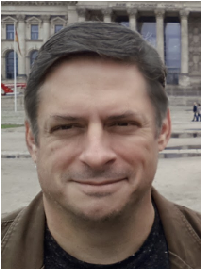
\includegraphics[width=3cm]{images/Soliday.eps}
\end{wrapfigure}

\textbf{Stephen W. Soliday, MSEE}--is a senior systems engineer and
research scientist with L-3 Advanced Defense Solutions.
He is responsible for providing subject matter expertise for Machine
Learning, Advanced Algorithms, and Cyber Autonomy. He is a member of
L3’s newly formed AI Community of Practice.  In 2015, Mr. Soliday was
elected as an L3-NSS Engineering Fellow.  In 1992, Mr. Soliday earned
a Bachelor’s degree in physics and mathematics, concentrating on
computational astrophysics. In 1996, Mr. Soliday completed a Master of
Science in Electrical Engineering with a concentration on Machine
Leaning and Controls. His research involved autonomous behavior for
mobile robotics on a research grant from DARPA. Mr. Soliday has worked
for Texas Instruments, Raytheon, Titan, and L3 Technologies. In the
mid-1980’s Mr. Soliday served in the U.S. Army Air Defense.
Mr. Soliday has over 25 years of technical expertise in the
application of Machine Learning and Autonomy to: information
operations, weapon systems, unmanned vehicles, and C4ISR systems, for
both National and DOD programs. He has implemented and supported
technologies such as genetic algorithms, fuzzy-logic, neural-networks,
intelligent-agents, and Kalman-filters, to advanced research projects,
concept development programs, and production systems.  Mr. Soliday has
supported, designed, and led many computational modeling and
simulation projects. 
